\subsection{Thế Giới Di Động}
\begin{figure}[H]
    \centering
    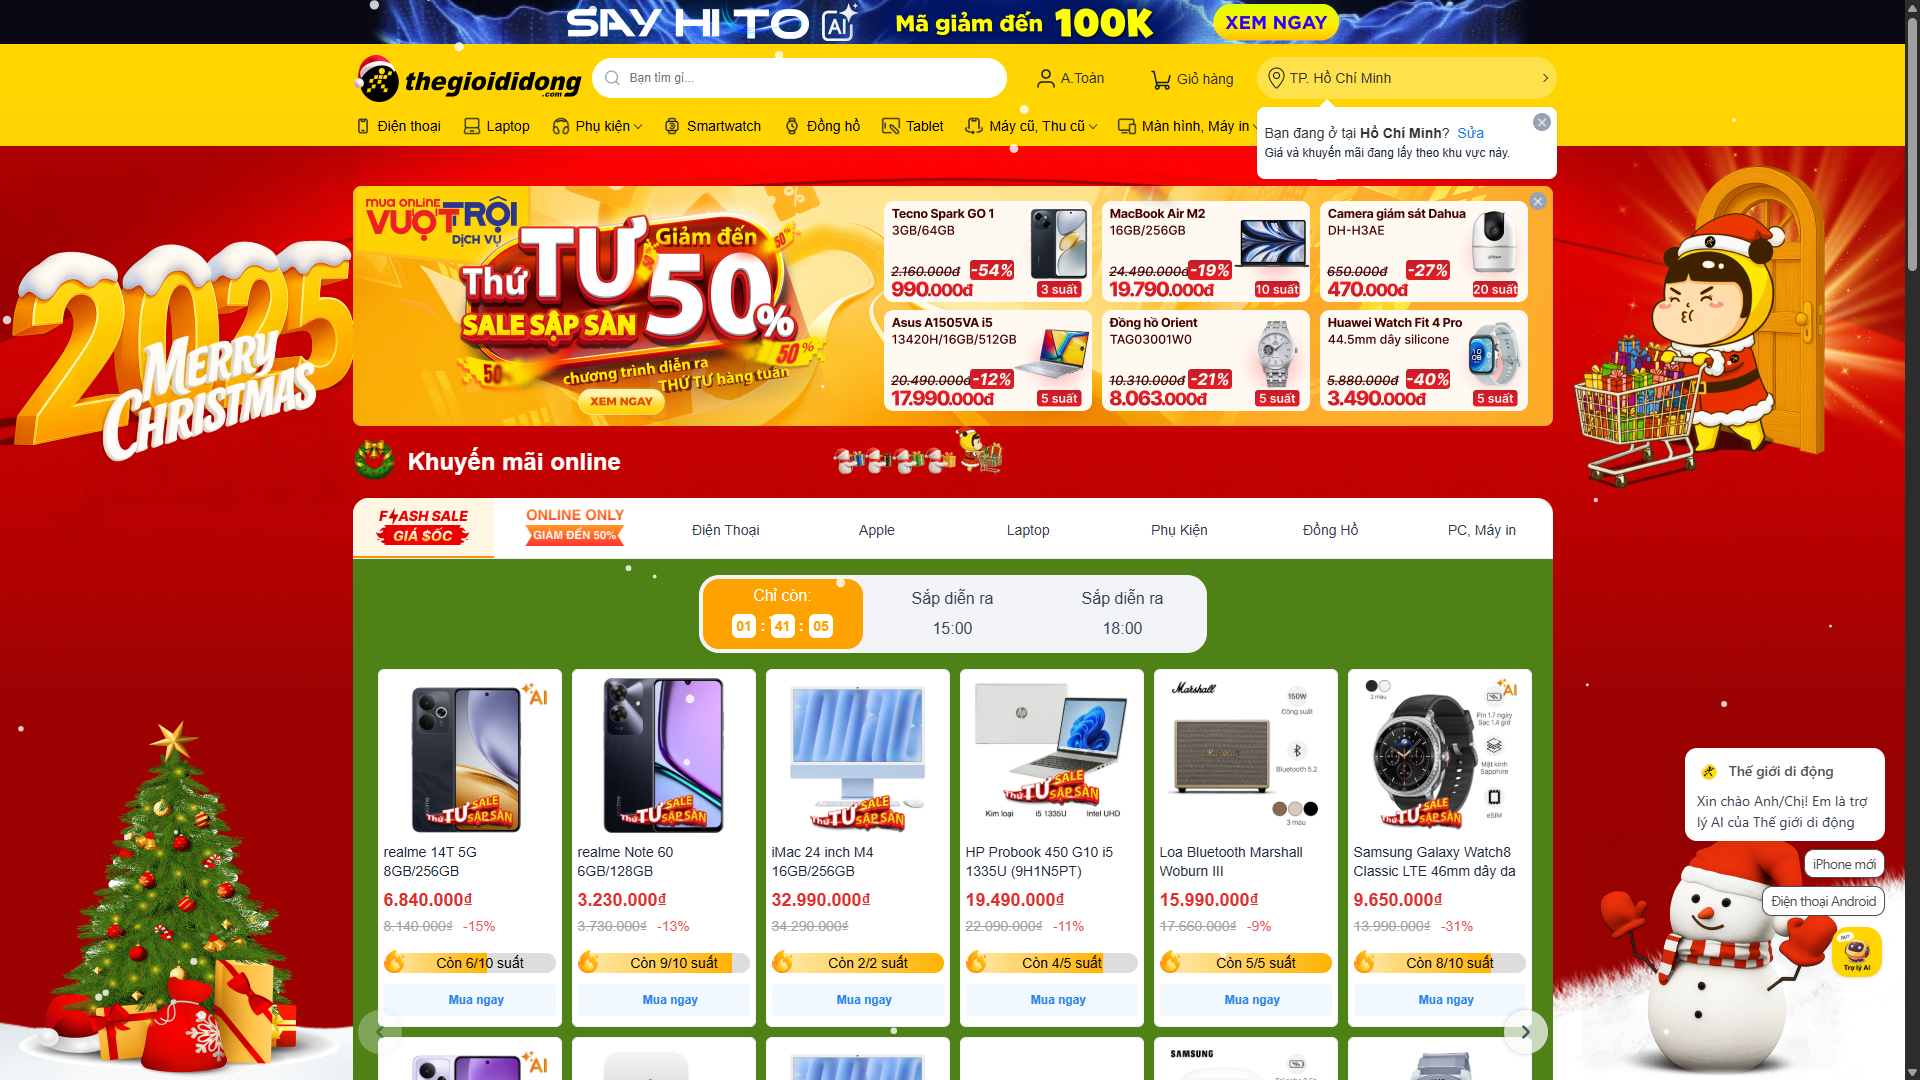
\includegraphics[width=\textwidth]{images/chap2/tgdd.png}
    \vspace{0.5cm}
    \caption{Trang chủ của Thế Giới Di Động}
\end{figure}

Thế Giới Di Động là hệ thống bán lẻ điện thoại và thiết bị điện tử tiêu dùng lớn nhất Việt Nam, với hàng nghìn cửa hàng trên toàn quốc. Website được tối ưu cho người dùng phổ thông, tập trung vào quy trình mua nhanh, khuyến mãi hấp dẫn và chính sách hậu mãi rõ ràng.

\textbf{Tính năng nổi bật:}
\begin{itemize}
    \item Bộ lọc sản phẩm đa tiêu chí, gợi ý kết quả tức thì và hiển thị sản phẩm nổi bật.
    \item Chính sách giao hàng, đổi trả, bảo hành minh bạch.
    \item Hệ thống khuyến mãi, flash sale và combo sản phẩm trình bày nổi bật.
    \item Hỗ trợ khách hàng đa kênh: hotline, chat trực tuyến, mạng xã hội và cửa hàng.
\end{itemize}

Website của Thế Giới Di Động có thiết kế thân thiện, tốc độ truy cập cao và khuyến mãi cập nhật liên tục. Bên cạnh đó, Thế Giới Di Động đã tích hợp trợ lý ảo hỗ trợ khách hàng. Tuy nhiên, các trợ lý ảo này chỉ dừng lại ở mức trả lời câu hỏi hoặc hướng dẫn cơ bản. Các trợ lý ảo này chưa làm tốt trong việc duy trì một luồng hỗ trợ khách hàng nhiều lượt và phi tuyến tính.

\begin{figure}[H]
\centering
\begin{minipage}{0.30\textwidth}
    \centering
    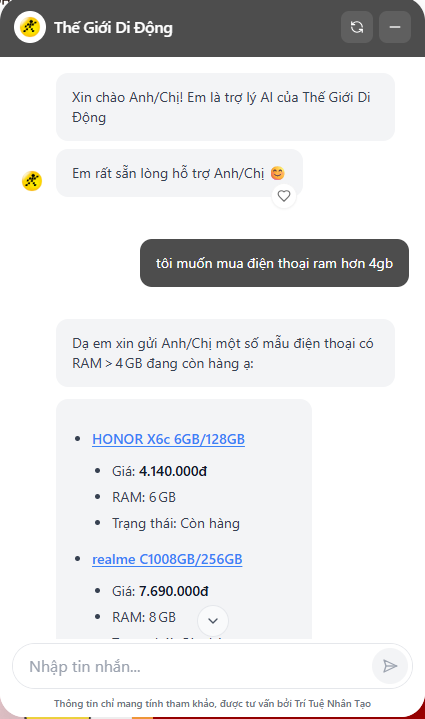
\includegraphics[width=0.8\textwidth]{images/chap2/tgdd_good.png}
\end{minipage}
\hfill
\begin{minipage}{0.30\textwidth}
    \centering
    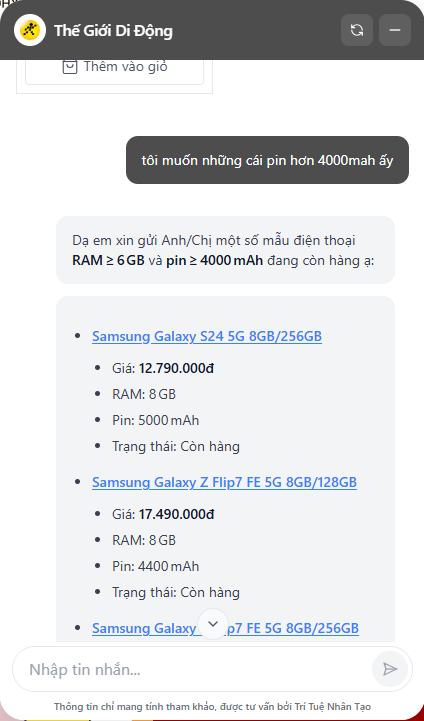
\includegraphics[width=0.8\textwidth]{images/chap2/tgdd_bad1.png}
\end{minipage}
\hfill
\begin{minipage}{0.30\textwidth}
    \centering
    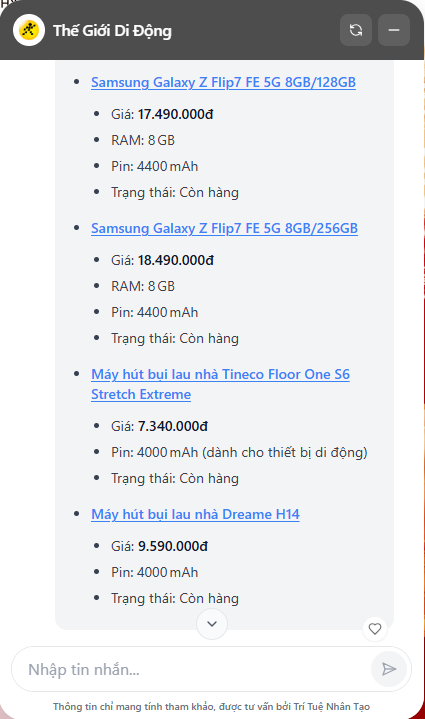
\includegraphics[width=0.8\textwidth]{images/chap2/tgdd_bad2.png}
\end{minipage}
\vspace{0.5cm}
\caption{Trợ lý ảo của Thế Giới Di Động}
\end{figure}
